\documentclass[11pt]{jarticle}
\usepackage{newcent}             % PDFへの変換後の品質を高める
\usepackage{listings,jlisting}
\usepackage{url}
\usepackage{float}
\usepackage[dvipdfmx]{graphicx}

%\usepackage[doctor]{gaiyo}      % 博士論文要旨の場合
%\usepackage[master]{gaiyo}      % 修士論文要旨の場合
%\usepackage{gaiyo}               % 卒業研究概要の場合
\usepackage[junior]{gaiyo}      % 専門演習レポートの場合

\lstset{%
  language={},
  basicstyle={\small},%
  identifierstyle={\small},%
  commentstyle={\small\itshape},%
  keywordstyle={\small\bfseries},%
  ndkeywordstyle={\small},%
  stringstyle={\small\ttfamily},
  frame={single},
  breaklines=true,
  columns=[l]{fullflexible},%
  numbers=left,%
  xrightmargin=0zw,%
  xleftmargin=3zw,%
  numberstyle={\scriptsize},%
  stepnumber=1,
  numbersep=1zw,%
  lineskip=-0.5ex%
}

\title{Python}
\id{情13-209}
\author{坂本 要}
\teacher{小林 孝史}

\begin{document}
\maketitle
\section{型}
プログラミングで使われるデータには「型」と呼ばれるものがある.例えば1や2は「数値」で"Hello"というテキストは「文字列」という型である.Pythonには様々なデータ型が用意されている.今回はその中でも重要な数値,文字列,Bool,リストについて説明する.
\subsection{数値型}
CやJavaでは「整数」と「少数」は別物であり,表現できる上限値が決まっている.Javaの整数型であるintは整数を表現する型であるため,小数点は扱うことができない.Pythonでも正確には整数型や少数型は存在するものの,それらは同じ「数値型」のようなイメージで扱うことが出来る.
%>>> 5 * 5
%25
%>>>5.5 *  5
%27.5
数値計算では表\ref{arithmetic operator}の演算子が利用可能である.
\begin{table}[h]
\centering
 \caption{算術演算子}
  \begin{tabular}{|c|c|} \hline
    操作 & 結果  \\ \hline \hline
    x + y & xとyの和 \\ \hline
    x - y & xとyの差 \\ \hline
    x * y & xとyの積 \\ \hline
    x / y & x割るyの商 \\ \hline
    x \% y & x割るyの余剰 \\ \hline
    x ** y & xのy乗 \\ \hline
  \end{tabular} 
 \label{arithmetic operator}
\end{table}

\subsection{文字列型}
文字列は'シングルクォーテーションか"ダブルクォーテーションで囲む.テキストも数値と同様に「+」を使うことで結合ができる
%>>> text = "Hello" + "Python"
%>>> print text
%Hello Python

\subsection{Bool型}
Boolは「真偽値」とも呼ばれる「True/False」の2値を持つ型である.Boolは表\ref{comparative operator}に示した比較演算子と呼ばれる記号で2つの値を比較した際に返される.
\begin{table}[h]
 \centering
   \caption{比較演算子}
    \begin{tabular}{|c|c|} \hline
     操作 & 意味 \\ \hline \hline
     x == y & xとyは等しい \\ \hline
     x != y & xとyは等しくない \\ \hline
     x < y & xはyより小さい \\ \hline
     x > y & xはyより大きい \\ \hline
     x <= y & xはy以下 \\ \hline
     x >= y & xはy以上 \\ \hline
    \end{tabular}
   \label{comparative operator}
\end{table}
%>>> 10 > 5
%True
%>>> 10 < 5
%False
%>>> a = 10 > 5
%>>> a
%>>>True


また,複数の比較演算子の結果を組み合わせて評価する場合,表\ref{logical operator}の論理演算子を用いる.
\begin{table}[h]
 \centering
  \caption{論理演算子}
   \begin{tabular}{|c|c|} \hline
   操作 & 意味 \\ \hline \hline
   not x & xが偽であれば真 \\ \hline
   x and y & xもyも真ならば真 \\ \hline
   x or y & xまたはyが真ならば真 \\ \hline
   \end{tabular}
  \label{logical operator}
\end{table}

%>>> not 10 < 5
%True
%>>> 10 == 10 and 5 == 5
%True
%>>> 10 < 5 or 10 > 5
%True

\subsection{リスト}
リスト型はデータを「リスト」状に複数個並べたような型である.リストを使わずに3人の学生の平均点を求めようとすると以下のようなコードがかける.
\begin{lstlisting}[basicstyle=\ttfamily\footnotesize, frame=single]
student1 = 68
student2 = 81
student3 = 49
average = (student1 + student2 + student3) / 3
print average
 \end{lstlisting}
このコードの場合,学生の人数が4人になった場合,修正する箇所が多いことが問題点としてあげられる.このような問題はリストを使うことである程度解消することが出来る.リストは「リストというデータの中に複数のデータを格納できる」という型なので,「学生達の点数」というデータに「具体的な各学生の点数」を格納する.
\begin{lstlisting}[basicstyle=\ttfamily\footnotesize, frame=single]
results = [68, 81, 49]
average = sum(results)/len(results)
print average
\end{lstlisting}
1行目で「学生たちの点数」というリストを作成している.2行目にあるsum()はリスト内にあるデータの合計値を算出する関数,len()はリストに格納されるデータの数を返す関数である.2つめのコードは学生一人ひとりの点数毎に変数を作成していないので,「複数の学生たちの点数の格納」が簡単なことに加え,平均値の算出方法が学生の数に依存していない.リストを使うことで「ひとつのグループに属するデータ」を便利に扱うことが出来る.
\begin{lstlisting}[basicstyle=\ttfamily\footnotesize, frame=single]
>>> a = []
>>> b = [1, 2, 3]
>>> c = [1, "2", False]
\end{lstlisting}
[]の中に何も入れない場合はからのリストを作成する.3行目のようにリストの中に様々なデータが入れられることには注意したい.リストの要素を取り出すにはリスト内のx番目の要素を指定する必要がある.
\begin{lstlisting}[basicstyle=\ttfamily\footnotesize, frame=single]
リスト名[要素の番号]
\end{lstlisting}
指定する順序は1からではなく0からである.
\begin{lstlisting}[basicstyle=\ttfamily\footnotesize, frame=single]
>>>b = [1,2,3]
>>>print(b[0]) # 1
>>>print(b[2]) # 3
>>>b[1] = 5
>>>print(b[1]) # 5
>>> b.append(4)   # 末尾への追加
>>> print(b)
[1, 2, 3, 4]
>>> b.insert(1,10)   # 1番目の要素に10を追加
>>> print(b)
[1, 10, 2, 3, 4]
>>> b = [1,2,3]
>>> b.remove(1)
>>> print(b)
[2, 3]
\end{lstlisting}

\section{分岐処理}
ifを使うことで条件に応じた分岐処理を行うことが可能である.ifに続く式が真であればインデントされたブロックの処理が実行される.複数の条件を指定する場合elifを用いる.elifは任意の数繰り返すことが可能である.いずれにも該当しない場合の処理はelseに続けて書くが,省略することも出来る.Bool型が条件判定に利用され,その値がTrueかFalseかで実行するプログラムが変わる.
\begin{figure}[h]
 \centering
  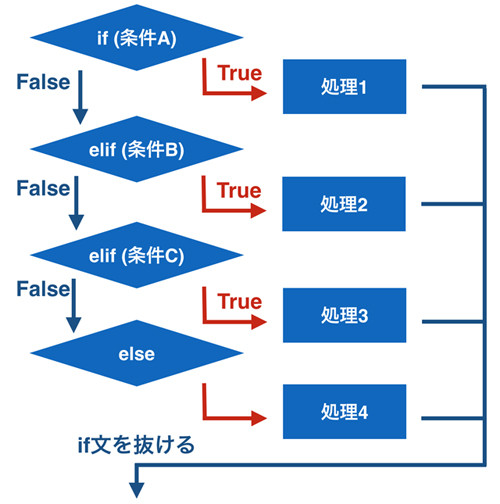
\includegraphics[width=9cm]{001.jpg}
  \caption{条件分岐の仕組み}
  \label{scale}
\end{figure}
\begin{lstlisting}[basicstyle=\ttfamily\footnotesize, frame=single]
if 条件A:
    処理1  # 条件 A が True の時に実行される処理
elif 条件B:
    処理2  # 条件 A が False で条件 B が True の時に実行される処理
elif 条件C:
    処理3  # 条件 A,B が False で条件 C が True の時に実行される処理
else:
    処理4  # 全ての条件が False の時に実行される処理
\end{lstlisting}
%標準入力を用いて入力した値が偶数か奇数かを判定するプログラムを作ってもらう?

\section{ループ処理}
ループ処理は「同じ処理を何度も繰り返す」という処理である.ループ処理の制御構造にはforとwhileの2つがある.
\subsection{while}
whileは条件が真である間,インデントされたブロックの処理を繰り返し実行する.
\begin{figure}[h]
 \centering
  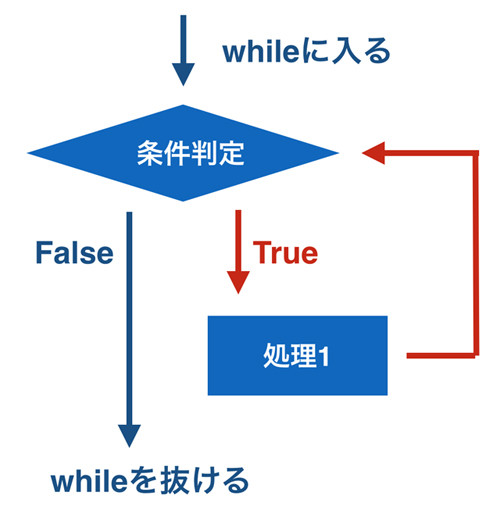
\includegraphics[width=9cm]{003.jpg}
  \caption{Pythonのwhile文}
  \label{scale}
\end{figure}

\newpage
\begin{lstlisting}[basicstyle=\ttfamily\footnotesize, frame=single]
 n = 0
 while n < 10:
 	print n
	n += 1
\end{lstlisting}
% +=の説明

\subsection{for}
forはグループにある要素を取り出し繰り返し処理を実行するといった時に使われる.リストに格納されている要素をすべてチェックするような処理でよく使われる
\begin{figure}[h]
 \centering
  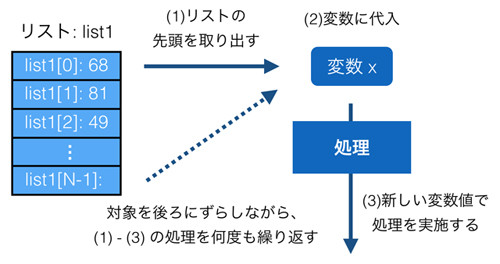
\includegraphics[width=12cm]{002.jpg}
  \caption{Pythonのfor文}
  \label{scale}
\end{figure}

\begin{lstlisting}[basicstyle=\ttfamily\footnotesize, frame=single]
 n = [1,2,3]
 for x in n:
 	print x 	# 1, 2, 3
\end{lstlisting}
range関数を使うことによって指定した回数だけ繰り返し処理を行うことも可能である.
\begin{lstlisting}[basicstyle=\ttfamily\footnotesize, frame=single]
 for x in range(10):
 	print x	# 0, 1, 2, 3, 4, 5, 6, 7, 8, 9
\end{lstlisting}
%forを用いて

\subsection{break}
whileやforを使った繰り返し処理はbreakを使うことで抜け出すことができる.
\begin{lstlisting}[basicstyle=\ttfamily\footnotesize, frame=single]
 for x in range(10):
 	if x == 5:
		break
	print x	# 0, 1, 2, 3, 4, 5
\end{lstlisting}
%whileを用いて1から1000までの数の和を求めるプログラムを作成せよ

\section{関数}
pythonには様々な組み込み関数が用意されている\cite{built-in}.これまで使用してきたraw\_input()やrange(),sum(),len()などがそれである.関数を利用する利点としてプログラムの可読性が向上することがあげられる.例えば絶対値を得ようと思った場合,以下のようにifを使って条件分岐させることで実現が可能である.
\begin{lstlisting}[basicstyle=\ttfamily\footnotesize, frame=single]
x = -5
if(x<0):
    x = x * -1
print(x)
\end{lstlisting}
同じ処理を組み込み関数であるabs()を使って書くと以下のようになる
\begin{lstlisting}[basicstyle=\ttfamily\footnotesize, frame=single]
x = abs(-5)
print(x)
\end{lstlisting}
関数には同じコードを何度も書かなくてすむといったメリットもある.
\begin{lstlisting}[basicstyle=\ttfamily\footnotesize, frame=single]
x = 5
y = -10

if(x<0):
    x = x * -1
if(y<0):
    y = y * -1

print 'abs x > abs y ?'
print x > y 
\end{lstlisting}
関数を使って書き直すと
\begin{lstlisting}[basicstyle=\ttfamily\footnotesize, frame=single]
x = 5
y = -10

x = abs(x)
y = abs(y)

print 'abs x > abs y ?'
print x > y
\end{lstlisting}
関数は自分で作成することも可能である.関数は入力を受け取り,それを加工して出力する.入力と出力はなくてもかまわず,入力がない場合は関数の宣言の引数をなくし,出力が不要な場合はreturn文をなくす.
\begin{lstlisting}[basicstyle=\ttfamily\footnotesize, frame=single]
# 引数がない関数
def my_func1():
  return 0

# 返り値がない関数
def my_func2(x):
  x = x * -1
\end{lstlisting}
関数は宣言した引数に対応する箇所に入力値を入れることで呼び出す.引数がない関数に関しては()に何も入れずに,引数を取る場合は()に値を入力する.
\begin{lstlisting}[basicstyle=\ttfamily\footnotesize, frame=single]
print my_func1()  # 0 と表示される
print my_func2(5) # None と表示される
\end{lstlisting}
引数は複数指定できるが,return文は一度しか実行されない.
\begin{lstlisting}[basicstyle=\ttfamily\footnotesize, frame=single]
def my_func3(x, y):
    print "A"
    if(x > y):
        return x
    print "B"
    return y

print my_func3(5,1)
# A
# 5

print my_func3(2,4)
# A
# B
# 4
\end{lstlisting}
上記のコードでは2つのreturn文が確認できる.x>yの条件が満たされた場合Bが出力されていないことに注目して欲しい.returnはいくつあっても構わないが,returnされたあとの関数の処理は一切無視される.
\subsection{グローバル変数とローカル変数}
\begin{lstlisting}[basicstyle=\ttfamily\footnotesize, frame=single]
x = 5
def square(x):
	return x * x
print x
square(10)
print x
\end{lstlisting}
\begin{thebibliography}{10}
\bibitem{built-in} 2. 組み込み関数 — Python 2.7.x ドキュメント,http://docs.python.jp/2/library/functions.html,2016年3月17日確認.
\end{thebibliography}
\end{document}